Die Variable \verb+participant+ ist für die Funktion des Algorithmus nicht
essentiell. Er würde auch funktionieren, wenn man das gesamte
\verb+if+-Statement durch 
\begin{verbatim}
  send <election, i> to successor;
\end{verbatim}
ersetzt.
Die Variable \verb+participant+ verhindert, dass nebenläufige Wahlvorgänge laufen. Kommt der zweite
Wahlvorgang beim Initiator der ersten Wahl an, dann wird dieser nicht weiter propagiert.
\\ \medskip
Der Algorithmus im Foliensatz 11 auf Seite 11 ist jedoch nicht korrekt. Durch den
\verb+else+-Zweig \verb+j=i+ kann es dazu kommen, dass nicht der Prozess mit der
höchsten ID zum Leader gewählt wird. Ausserdem kann es passieren, dass zur
gleichen Zeit zwei unterschiedliche Knoten für unterschiedliche Leader stimmen, was nach
Voraussetzung nicht passieren darf. \\
Im folgenden Beispiel starten 2 Knoten den Wahlalgorithmus (Knoten 2 und kurz
danach Knoten 1) (siehe \ref{fig:9_1_1}). Bekommt nun Knoten 2 die
\verb+election+-Nachricht von Knoten 1, sendet Knoten 2 eine \verb+<elected, 2>+-Nachricht 
(siehe \ref{fig:9_1_2}). Auch Knoten 3 aktzeptiert die Wahl von Knoten 2 und leitet die
Nachricht weiter. Kurz darauf kommt jedoch die Nachricht \verb+<election, 3>+ 
wieder bei 3 an (von der von 2 initierten Wahl) und 3 sendet seinerseit eine
\verb+<elected, 3>+-Nachricht. Es werden also während der Abarbeitung des Algorithmus 2 unterschiedliche Leader gewählt
(siehe \ref{fig:9_1_3}), was nach Vereinbahrung am Anfang des Foliensatz 11 nicht zulässig ist. 
\begin{figure}
  \begin{center}
    \includegraphics{./pics/9_1_1}
  \end{center}
  \caption{Knoten 2 startet eine Wahl und kurz danach auch Knoten 1}
  \label{fig:9_1_1}
\end{figure}

\begin{figure}
  \begin{center}
    \includegraphics{./pics/9_1_2}
  \end{center}
  \caption{Der falsche else-Zweig wird ausgeführt}
  \label{fig:9_1_2}
\end{figure}

\begin{figure}
  \begin{center}
    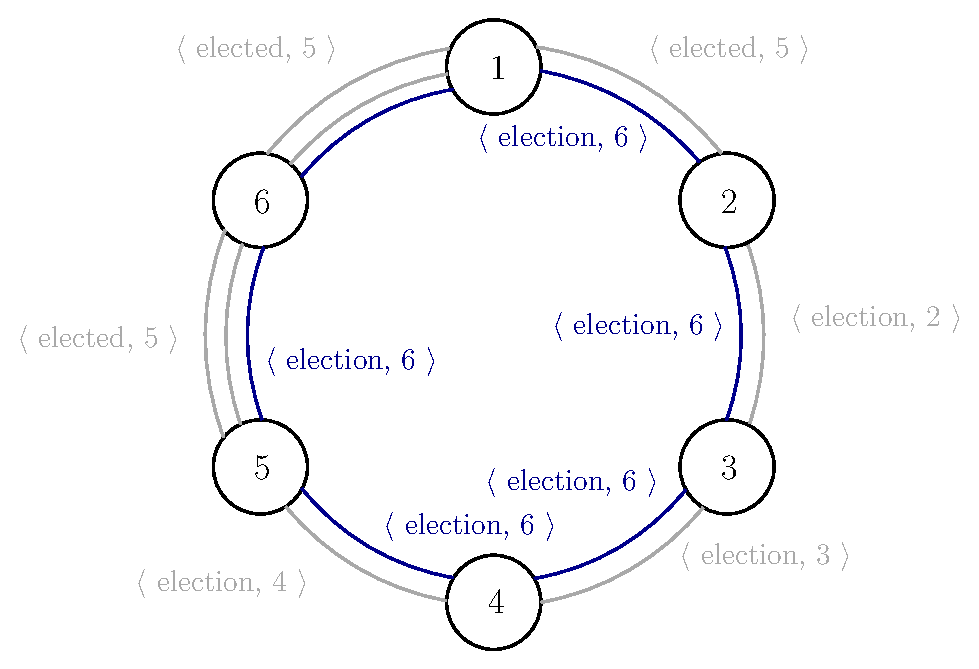
\includegraphics{./pics/9_1_3}
  \end{center}
  \caption{Zwei Knoten haben unterschiedliche Leader gewählt}
  \label{fig:9_1_3}
\end{figure}
